
%(BEGIN_QUESTION)
% Copyright 2006, Tony R. Kuphaldt, released under the Creative Commons Attribution License (v 1.0)
% This means you may do almost anything with this work of mine, so long as you give me proper credit

Anta at du ser denne merkingen på en kjemikaliebeholder:

$$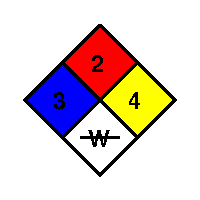
\includegraphics[width=15.5cm]{i00585x01.eps}$$

Dette er en standardisert etikett (National Fire Protection Association -- NFPA) som angir visse farer ved kjemikaliet i beholderen. Forklar hva alle markeringene betyr.

\underbar{file i00585}
%(END_QUESTION)





%(BEGIN_ANSWER)

Dette kjemikaliet er klassifisert som ``svært farlig'', med flammepunkt mellom 100$^{o}$F og 200$^{o}$F, og kan detonere under normale forhold. I tillegg er det farlig ved kontakt med vann.

\vskip 10pt

Venstre (blå) diamant angir helsefare:

\begin{itemize}
\item{} 0 = Ingen fare
\item{} 1 = Lett fare
\item{} 2 = Moderat farlig
\item{} 3 = Svært farlig
\item{} 4 = Dødelig
\end{itemize}

\vskip 10pt

Øvre (rød) diamant angir brennbarhet (flammepunkt):

\begin{itemize}
\item{} 0 = Brenner ikke
\item{} 1 = Over 200$^{o}$F
\item{} 2 = Mellom 100$^{o}$F og 200$^{o}$F
\item{} 3 = Mellom 73$^{o}$F (romtemperatur) og 100$^{o}$F
\item{} 4 = Under 73$^{o}$F (romtemperatur)
\end{itemize}

\vskip 10pt

Høyre (gul) diamant angir kjemisk reaktivitet:

\begin{itemize}
\item{} 0 = Stabil
\item{} 1 = Ustabil ved oppvarming
\item{} 2 = Kraftig kjemisk endring, men ingen detonasjon
\item{} 3 = Sjokk eller varme kan detonere
\item{} 4 = Kan detonere under normale forhold
\end{itemize}

\vskip 10pt

Nedre (hvit) diamant brukes for tilleggsopplysninger. Standardforkortelser inkluderer:

\begin{itemize}
\item{} ACID = Sur
\item{} ALK = Alkalisk
\item{} COR = Etsende
\item{} OX = Oksiderende
\item{} P = Polymerisering
\item{} W (med strek gjennom) = Reagerer med vann
\end{itemize}

%(END_ANSWER)





%(BEGIN_NOTES)

%INDEX% Kjemi, sikkerhet: NFPA-faremerking

%(END_NOTES)

